 \section{NP-hard problems for Sullivan algebras} \label{sec:NPSullivan}
 
 In this section we show the 
 $\NPcomplexity$-hardness of computing certain properties of Sullivan algebras. This will directly 
 translate to the $\NPcomplexity$-hardness of computing topological invariants.
 The theorems and proofs in this section mainly follow  \cite{Lechuga2000} and
 \cite{Garvin2003}. Throughout this section the ground ring of all modules and algebras
 will be $\Q$.


 \begin{Definition}
  A Sullivan algebra $(\Lambda V, d)$ is called \emph{elliptic} if both $V$ and $H(\Lambda V,d)$ have
  finite dimension.
 \end{Definition}
 
 The main result we want to establish is the following:
 
 \begin{Theorem}[Lechuga, Murrilo]
 \label{thm:DecidingEllipticityIsNpHard}
  It is a $\NPcomplexity$-hard problem to decide if a given Sullivan algebra $(\Lambda V,d)$ with $V = { \{ V^n \} }_{n \geq 2}  $ finite dimensional 
  is elliptic . 
 \end{Theorem}
 
 \begin{Remark}
 \label{rem:CodingOfSullivanAlgebras}
  To be able to speak about complexity of computations involving Sullivan algebras we first have to fix a bit string 
  representation of a Sullivan algebra. However, Sullivan algebras could have infinitely many generators and would therefore
  not be representable in a computer. Thus, we stick to Sullivan algebras $\Sullivan$ where $V$ is finite dimensional. 
  We encode such an algebra $(\Lambda V, d)$ with $V = \langle v_1, \ldots , v_n \rangle$
  by the following string: \newline
  Fix the smallest $c \in \N$ such that $d(V) \subseteq \Lambda^{ \leq c} V$.
  The first part of the string consists of 
  an $n$-tuple of integers encoding the degrees of the $n$ generators. This is linear in the number
  of generators. Then add for each $ 1 \leq i \leq n$
  and $d v_i = \sum_{q \leq c, (j_1, \ldots, j_q)} \lambda_{j_1, \ldots, j_q} v_{j_1} \cdots v_{j_q}$ all tuples 
  $(({j_1, \ldots, j_q}), \lambda_{j_1, \ldots, j_q})$ storing the indices and the rational coefficient 
  $\lambda_{j_1, \ldots, j_q}$ (which is represented by two integers) to the string. \\
  Let $k$ be the number of integers stored in all these tuples. We have $n$ generators,
  ${ n \choose q}$ choices of $q$ generators out of $n$ and at most $c + 2$ integers per tuple. Therefore, we can bound $k$ by
  $k \leq (c + 2)n \sum_{q = 1}^c { n \choose q} $ and this is polynomial in $n$ for fixed $c$.
  Hence, if $c$ is fixed the representation has polynomial length in the number
  of generators.
  
 \end{Remark}

 The next pages will be dedicated to proving \ref{thm:DecidingEllipticityIsNpHard}.
 The main idea of the proof is to reduce $k$-COLOUR to deciding if $(\Lambda V,d)$ is elliptic for some special 
 Sullivan algebra $(\Lambda V,d)$ which we construct as follows: \\
 
 \begin{Construction}
 \label{constructionOfSullivanAlgebra}
 Let $G = (V,E)$ be an undirected, simple, connected, finite graph with vertices $ V = \lbrace v_1, \dotsc , v_n \rbrace $
 and edges $ E = \lbrace (v_r, v_s) \; | \; (r,s) \in J \rbrace$. We construct for $k \geq 2$ the 
 Sullivan algebra $(\Lambda V_{(G,k)} , d)$ as follows: \\
 
 $ V^{even}_{(G,k)} \coloneqq \langle x_1, \dotsc , x_n \rangle $ \; with \; $|x_i| = 2$ \; for \; $ i = 1, \dotsc , n$ \; 
 and \; $dx_i \coloneqq 0$ \\
 
 $V^{odd}_{(G,k)} \coloneqq \langle y_{(r,s)} \rangle$ , $(r,s) \in J$ \; with \; $|y_{(r,s)}| = 2k - 3$ \; and \; $dy_{(r,s)} \coloneqq 
 \sum_{l = 1}^k x_r^{k -l} x_s^{l - 1}$ \\
 
 \end{Construction}

\begin{Remark}
  The algebras constructed above are all pure. For 
  $k \geq 3$ all $dy_{(r,s)}$ contain no linear term, hence
  $(\Lambda V_{(G,k)} ,d)$ is minimal for $k \geq 3$.
  The vector space
  $V_{(G,k)}$ has as many generators as $G$ has vertices. Thus, by Remark \ref{rem:CodingOfSullivanAlgebras}
  the representation of $(\Lambda V_{(G,k)} ,d)$ is for fixed $k$ polynomial in the number of edges and vertices of $G$ .
%   
%   The construction
%   is for $k$ fixed polynomial in the number of vertices since the constructed vector space
%   $V_{(G,k)}$ has as many generators as $G$ has vertices and Remark \ref{rem:CodingOfSullivanAlgebras}
%   shows that the representation of $(\Lambda V_{(G,k)} ,d)$ is polynomial in $dim \, V_{(G,k)}$.
%   
\end{Remark}

\begin{Example}
 Without being aware of it, we already have seen examples of Sullivan 
 algebras constructed by \ref{constructionOfSullivanAlgebra}. For this, consider the following
 graphs:
 
 \begin{multicols}{2}
  \begin{tikzpicture}[auto, node distance=2cm, every loop/.style={},
                    main node/.style={circle,draw,font=\sffamily\Large\bfseries}]

  \node[main node] (a) {a};
  \node[main node] (b) [below left of=a] {b};
  \node[main node] (c) [below right of=a] {c};

  \path[every node/.style={font=\sffamily\small}]

    (a) edge node [right] {z} (c)
	 edge node [left] {x} (b)

	(b) edge node [below] {y} (c)	;


    \node [below=2.5cm, align=flush center,text width=8cm] at (a)
        {
             $K_3$
        };


\end{tikzpicture}

\columnbreak

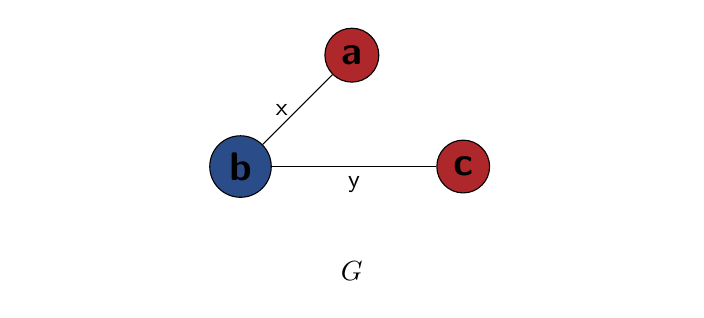
\begin{tikzpicture}[auto, node distance=2cm, every loop/.style={},
                    main node/.style={circle,draw,font=\sffamily\Large\bfseries}]

  \node[main node, fill = {rgb:red,219;green,50;blue,54}] (a) {a};
  \node[main node, fill = {rgb:red,72;green,133;blue,237}] (b) [below left of=a] {b};
  \node[main node, fill = {rgb:red,219;green,50;blue,54}] (c) [below right of=a] {c};

  \path[every node/.style={font=\sffamily\small}]

    (a) edge node [left] {x} (b)

	(b) edge node [below] {y} (c)	;


    \node [below=2.5cm, align=flush center,text width=8cm] at (a)
        {
            $G$
        };


\end{tikzpicture}

 \end{multicols}

 If we apply construction \ref{constructionOfSullivanAlgebra} for $k=2$ to $K_3$ we get the Sullivan algebra $\Sullivan$
 from example \ref{ex:AlgebraConstructedFromK3}. We have seen that it has finite dimensional homology. Further, 
 applying the construction to $G$ yields the Sullivan algebra $\Sullivan$ from example \ref{ex:AlgebraFromK3WithoutOneEdge} which
 has infinite dimensional homology. Note that $G$ is 2-colourable (as indicated in the picture) while
 $K_3$ is not.
\end{Example}

This relation between $k$-colourabilty and infinite dimensional homology is not a coincidence as we shall see in

 \begin{Theorem}
 \label{thm:KColourEquivalentToNonEllipticity}
  Let $k \geq 2$ then 
   $G = (V,E)$ is k-colourable if and only if $(\Lambda V_{(G,k)},d)$ is not elliptic
 \end{Theorem}
 
 First, we need a somehow technical Lemma:
 \begin{Lemma}
 \label{lma:IfAndOnlyIfNonTrivialMorphism}
  Let $\K$ be an algebraically closed field and $(\Lambda V,d)$ a minimal Sullivan
  algebra over $\K$ with finite dimensional $V = {\lbrace V^n \rbrace}_{n \geq 2}$. \\ Then
  $H\Sullivan$ has finite dimension if and only if   
  the only morphism of differential graded algebras 
  $$ \varphi : \Sullivan \to (\K[\alpha],0) \; \text{ with $|\alpha| = 2$} $$ 
  is the trivial one.
 \end{Lemma}
  
  We postpone the proof of this Lemma and make the following observation:
  
 
\begin{Lemma}
\label{lma:cohomoly+equations}
 $H(\Lambda V_{(G,k)}, d)$ has infinite dimension if and only if the system of equations \\
 \begin{equation}
 \label{systemofequations}
 {\lbrace \sum_{l = 1}^k u_r^{k - l} u_s^{l - 1} = 0 \; | \; (r,s) \in J \rbrace}  
 \end{equation}
 
 has a non-trivial solution 
 $(\lambda_1 , \dotsc, \lambda_n) \in \C^n$
\end{Lemma}

\begin{proof}
 Note that by the universal coefficient theorem (\ref{thm:Universalcoefficients}) we have
 $$ H ((\Lambda V_{(G,k)}) \otimes \C, d) \cong H(\Lambda V_{(G,k)}, d) \otimes \C $$ 
 which implies that $(\Lambda V_{(G,k)}, d)$ as  $\Q$-algebra has finite dimensional homology if and only if
 ${((\Lambda V_{(G,k)}) \otimes \C , d)}$ has finite dimensional homology as $\C$-algebra. Then by
 Lemma \ref{lma:IfAndOnlyIfNonTrivialMorphism} $H(\Lambda V_{(G,k)},d)$  has infinite dimension if and only if 
 there is a non-trivial morphism of differential graded algebras 
 ${\varphi \colon (\Lambda V_{(G,k)} \otimes \C,d)  \to ( \C [\alpha] ,d' = 0)}$ with $|\alpha| = 2$. How must such a morphism look like?
 Clearly it must satisfy $\varphi(x_i) = \lambda_i \alpha$ for some $\lambda_i \in \C$ and $\varphi(y_{(r,s)}) = 0$ for all $(r,s) \in J$  since 
 $(\C [\alpha] , 0)$ is zero in odd degrees. Furthermore, $\varphi$ must commute with the differentials. Hence, 
 for all $(r,s) \in J$
 $$ 0 = d' \varphi(y_{(r,s)}) = \varphi(dy_{(r,s)}) = \varphi(\sum_{l = 1}^k x_r^{k -l} x_s^{l - 1})
 = \sum_{l = 1}^k \varphi(x_r)^{k -l} \varphi(x_s)^{l - 1}$$
 
 This shows that $(\varphi(x_i))_{i = 1, \dotsc , n}$ must be a solution of \ref{systemofequations}, which is non-trivial
 if $\varphi$ is non-trivial.
 This also works the other way round and every non-trivial solution  $(\lambda_1 , \dotsc, \lambda_n)$ of \ref{systemofequations}
 defines a non-trivial morphism by $\varphi(x_i) \coloneqq \lambda_i \alpha$ and $\varphi(y_{(r,s)}) \coloneqq 0$.
 \end{proof}

 The proof of \ref{thm:KColourEquivalentToNonEllipticity} will essentially use that a $k$-colouring
 of a graph can be translated to a solution of \ref{systemofequations} by using the colouring
 as exponents for a $k$-th root of unity.
 We demonstrate this at a concrete example before doing the general case.
  \begin{Example}
   Given the graph $G$
   \begin{center}
    

   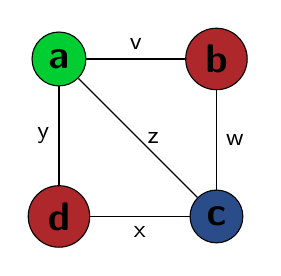
\begin{tikzpicture}[auto, node distance=2cm, every loop/.style={},
                    main node/.style={circle,draw,font=\sffamily\Large\bfseries}]

  \node[main node] (a)  [fill = {rgb:red,0;green,153;blue,37}] {a};
  \node[main node] (b) [right of=a, fill = {rgb:red,219;green,50;blue,54}] {b};
  \node[main node] (c) [below  of=b, fill = {rgb:red,72;green,133;blue,237}] {c};
  \node[main node] (d) [below  of=a, fill = {rgb:red,219;green,50;blue,54}]  {d};

  \path[every node/.style={font=\sffamily\small}]

    (a) edge node [left] {y} (d)
	 edge node [above] {v} (b)
	edge node [right] {z} (c)

	(b) edge node [right] {w} (c)	

	(c) edge node [below] {x} (d);




\end{tikzpicture}
   \end{center}

with the indicated $3$-colouring we construct the Sullivan algebra 
\begin{align*} 
(\Lambda V_{(G,3)},d) \cong &\Lambda(a_2,b_2,c_2,d_2,v_3,w_3,x_3,y_3,z_3 ; dv = a^2 + ab + b^2, dw = b^2 + bc + c^2, \\
 &dx = c^2 + cd + d^2, dy = d^2 + ad + a^2 , dz = a^2 + ac + c^2)
\end{align*}
Since $G$ is $3$-colourable $(\Lambda V_{(G,3)},d) \otimes \C$  should have a non-trivial morphism to
$( \C[\alpha_2], 0)$. The idea to use the colour of a vertex as exponent of a fixed $k$-th root of unity looks 
concretely in this case as follows:
Let $\zeta_3 \in \C$ be a third unit root. Define a morphism of graded algebras
$\varphi \colon \Lambda V_{(G,3)} \to \C [ \alpha_2]$ by 
\begin{align*}
\varphi(a) = 1 = \zeta_3^3 & & \varphi(b) = \varphi(d) = \zeta_3 = \zeta_3^1&  & \varphi(c) = \zeta_3^2 & &
\text{$\varphi(\xi) = 0$ for $\xi \in \lbrace v,w,x,y,z \rbrace$} 
\end{align*}
using the universal property of the free commutative algebra. Note that we have associated the same exponent
to vertices with the same colour.
One can now check that $\varphi$ commutes with the differentials and therefore defines a non-trivial morphism of differential graded algebras
$\varphi \colon (\Lambda V_{(G,3)}, d) \to (\C [ \alpha_2],d' = 0)$. We exemplary check this on one generator:
$$d'\varphi(v) = 0 = 1 + \zeta_3 + \zeta_3^2 = \varphi( a)^2 + \varphi( a)\varphi(b) + \varphi ( b)^2 = 
\varphi(a^2 + ab + b^2) = \varphi( du)$$
and the same works for $w,x,y$ and $z$. 
  \end{Example}

\begin{Remark}
 If we added a new edge $ u = \lbrace b,d \rbrace$ to the graph $G$ from last example we would end up with the graph $K_4$ 
 \begin{center}
    

   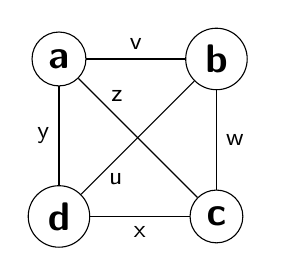
\begin{tikzpicture}[auto, node distance=2cm, every loop/.style={},
                    main node/.style={circle,draw,font=\sffamily\Large\bfseries}]

  \node[main node] (a)  [] {a};
  \node[main node] (b) [right of=a] {b};
  \node[main node] (c) [below  of=b] {c};
  \node[main node] (d) [below  of=a]  {d};

  \path[every node/.style={font=\sffamily\small}]

    (a) edge node [left] {y} (d)
	 edge node [above] {v} (b)
	edge node [above = 15, left = 2] {z} (c)

	(b) edge node [right] {w} (c)
	    edge node [below=15, left = 2]  {u} (d)

	(c) edge node [below] {x} (d);




\end{tikzpicture}
   \end{center}

 which
 is not $3$-colourable. Accordingly, if we extended the algebra $(\Lambda V_{(G,3)},d)$ from last example to the algebra
 $(\Lambda V_{(K_4,3)}, d)$ by adding one new generator $u_3$ with $du = b^2 + bd + d^2$ the analogous construction of $\varphi$ would
 not commute with the differentials since
 $$ \varphi(du) = \varphi(b)^2 + \varphi(b)\varphi(d) + \varphi(d)^2 = \zeta_3^2 + \zeta_3^2 + \zeta_3^2 = 3 \zeta_3^2 
 \neq 0 = d' \varphi(u)$$ 
 This corresponds to what we should expect from Theorem \ref{thm:KColourEquivalentToNonEllipticity}.
\end{Remark}

 
 \begin{proof}[proof of \ref{thm:KColourEquivalentToNonEllipticity}]
  From the construction of $(\Lambda V_{(G,k)},d)$ we see that  $V_{(G,k)}$ is finite dimensional, therefore
  it is elliptic if and only if its homology is finite dimensional. Suppose that $G$ is $k$-colourable and we are given a colouring
  $f \colon V \to { \lbrace 1, \dotsc , k \rbrace }$ with $f(x_r) \neq f(x_s)$ for $(r,s) \in J$. Let $\zeta_k$ be a primitive 
  $k$-th root of unity. For $(r,s) \in J$ it holds that
  
  $$ \sum_{l = 1}^k (\zeta_k^{f(x_r)})^{k-l} (\zeta_k^{f(x_s)})^{l-1}
  = \frac{(\zeta_k^{f(x_r)})^{k} - (\zeta_k^{f(x_s)})^{k}}{ \zeta_k^{f(x_r)} - \zeta_k^{f(x_s)}} = 0
  $$
  
  Hence $(\zeta_k^{f(x_i)})_{i = 1, \dotsc, n}$ defines a non-trivial solution of \ref{systemofequations}
  and Lemma \ref{lma:cohomoly+equations} tells us that $(\Lambda V_{(G,k)},d)$ is not elliptic. \\
  Let now $(\Lambda V_{(G,k)},d)$ be non elliptic. Then Lemma \ref{lma:cohomoly+equations} gives us a non-trivial
  solution $(\lambda_1 , \dotsc, \lambda_n) \in \C^n$ of \ref{systemofequations}. We use this solution to construct
  a colouring of $G$. 
  First observe that $\lambda_i \neq 0$ for all $i$: For this suppose that $\lambda_r = 0$ and let $(r,s) \in J$.
  We then have 
  $$0 =\sum_{l = 1}^k \lambda_r^{k -l} \lambda_s^{l - 1} = \lambda_s^{k-1}$$
  and hence $\lambda_s = 0$. Since G is connected this implies that all $\lambda_i$ are zero which is a
  contradiction to $(\lambda_1, \ldots, \lambda_n)$ being non-trivial.
  
  Next we have
  for $(r,s) \in J$ that
  
  $$ \lambda_r^k - \lambda_s^k = ( \lambda_r - \lambda_s) 
  \sum_{l = 1}^k \lambda_r^{k - l} \lambda_s^{l - 1} = 0$$
  
  Since $G$ is connected this implies
  $\lambda_1^k = \dotsc = \lambda_n^k$.  We can wlog assume that  $\lambda_1^k = 1$. Therefore, every $\lambda_i$ is a 
  $k$-th root of unity and we can define $f \colon V \to { \lbrace 1, \dotsc , k \rbrace }$ such that 
  $\lambda_i = \zeta_k^{f(x_i)}$.
  Assume that $f(x_i) = f(x_j)$ for some $(i,j) \in J$.
  From this we also get that 
  $$\sum_{l = 1}^k \lambda_i^{k - l} \lambda_j^{l - 1} = \sum_{l = 1}^k (\zeta_k^{f(x_i)})^{k-l} (\zeta_k^{f(x_j)})^{l-1}
  = \sum_{l = 1}^k (\zeta_k^{f(x_i)})^{k-1} = k (\zeta_k^{f(x_i)})^{k-1} \neq 0$$ 
  which is a contradiction to $(\lambda_1 , \dotsc, \lambda_n)$ being a solution of \ref{systemofequations}. Hence,
  $f(x_i) \neq f(x_j)$ for all $(i,j) \in J$.
  
 \end{proof}

 Having this at hand, the proof of \ref{thm:DecidingEllipticityIsNpHard} is just combining the above lemmata. We 
 shall prove a even stronger result as follows:
 
 Denote by $\Gamma_k$ the class of minimal Sullivan algebras $\Sullivan$ with $V$ finite dimensional and
 $d(V) \subset \Lambda^{< k} V$.
 
 \begin{Theorem}
 \label{thm:GammaKTheorem}
  For a fixed integer $k \geq 3$, deciding if a Sullivan algebra $\Sullivan \in \Gamma_k$ is elliptic is $\NPcomplexity$-hard. 
 \end{Theorem}

 \begin{Remark}
  
 Clearly \ref{thm:GammaKTheorem} directly implies \ref{thm:DecidingEllipticityIsNpHard}.
  
 \end{Remark}
 \begin{proof}
  Fix $k \geq 3$ and note that $k$-COLOUR is still $\NPcomplexity$-hard if we restrict it to connected graphs (since different
  components of a graph can be coloured independently). Given an undirected connected graph $G$ we use
  construction \ref{constructionOfSullivanAlgebra} and obtain the Sullivan algebra $(\Lambda V_{(G,k)},d)$ which lies
  in $\Gamma_k$ by construction. Further, by Remark \ref{rem:CodingOfSullivanAlgebras} this construction is polynomial
  in the number of vertices of $G$ and by Theorem \ref{thm:KColourEquivalentToNonEllipticity} deciding wether
  $(\Lambda V_{(G,k)},d)$ is elliptic is equivalent to deciding if $G$ is $k$-colourable. This means that if we can 
  decide if a given $\Sullivan \in \Gamma_k$ is elliptic we can also decide (with polynomial overhead) if a connected
  graph is $k$-colourable.
  \end{proof}

  For these classes $\Gamma_k$ of Sullivan algebras finite homology is equivalent to finite 
  category by \ref{prop:EquivalenceFiniteDimensionCategoryCohomology}, hence we directly get:
  
  \begin{Corollary}
   For fixed $k \geq 3$, computing $cat \, \Sullivan$ of a given $\Sullivan \in \Gamma_k$ is $\NPcomplexity$-hard.
  \end{Corollary}

  
  We still have to prove Lemma \ref{lma:IfAndOnlyIfNonTrivialMorphism} to complete the whole argumentation above. For the proof
  we have to cite the following theorem:
  
  \begin{Theorem}[Mapping Theorem for Sullivan algebras]
  \label{thm:MappingTheorem}
   Let $\varphi \colon \Sullivan \to (\Lambda W,d)$ be a surjective morphism of minimal Sullivan algebras with $V = V^{\geq 2}$
   and $W = W^{\geq 2}$ then $cat \Sullivan \geq cat(\Lambda W,d)$.
  \end{Theorem}
  \begin{proof}
   See \cite{Felix2001} Theorem 29.5.
  \end{proof}

  
  
 \begin{proof}[Proof of Lemma \ref{lma:IfAndOnlyIfNonTrivialMorphism}]
 
  
  Suppose that $H\Sullivan$ has finite dimension. A slight modification of Proposition \ref{prop:WellBehavedFiltrations} tells us that we can 
  choose a basis $v_1, \ldots , v_n$ of $V$ such that $d v_i \in \Lambda \langle v_1, \ldots, v_{i-1} \rangle$.
  Next, suppose we have a morphism  $ \varphi : \Sullivan \to (\K[\alpha],0)$ with  $|\alpha| = 2 $. We show by induction over $k$ that
  $\varphi$ is zero on $v_1 , \ldots, v_k$.
  For this, assume that $\varphi$ is zero on $v_1, \ldots, v_{k-1}$ then take the
  subalgebra of $\Sullivan$ induced by factoring out $v_1, \ldots, v_{k-1}$ and consider the induced morphism 
  $\bar{\varphi} \colon (\Lambda \langle \bar{x}_k, \ldots, \bar{x}_n \rangle , \bar{d}) \to (\K[\alpha],0) $
  (note that $\bar{d}(\bar{x}_k) = 0$ by the  choice of basis). Since $\K[\alpha]$ is zero in odd degrees,
  it follows that $\varphi(x_k) = 0$ for $|x_k|$ odd. If $|x_k|$ is even,
  it follows from \ref{prop:EquivalenceFiniteDimensionCategoryCohomology} and \ref{thm:MappingTheorem} 
  that $(\Lambda \langle \bar{x}_k, \ldots, \bar{x}_n \rangle , \bar{d})$ has finite category which gives us  $m \in \N$ and the
  following diagram
  
  \centerline {
  \xymatrix{
    (\Lambda \langle \bar{x}_k, \ldots, \bar{x}_n \rangle , \bar{d}) \ar@/^/[r]^(.45){\lambda_m} \ar[rd]_{\pi_m}	& 	
    (\Lambda \langle \bar{x}_k, \ldots, \bar{x}_n \rangle \otimes \Lambda Z(m) , d) 
    \ar[d]^{\zeta_m}_{\simeq} \ar@/^/[l]^{i_m} \\
    & (\Lambda \langle \bar{x}_k, \ldots, \bar{x}_n \rangle / 
    \Lambda^{> m} \langle \bar{x}_k, \ldots, \bar{x}_n \rangle, \tilde{d})
  }
  }
  It allows us to show that $\bar{x}_k^m$ is a coboundary as follows:
  Since the diagram commutes we have
  $$0 = \pi_m(\bar{x}_k^m) =   \zeta_m (\lambda_m (\bar{x}_k^m))$$ 
   Since $\zeta_m$ is a quasi isomorphism (and $\bar{x}_k^m$ a cocycle), we get that $\lambda_m (\bar{x}_k)$ is a coboundary and
  therefore also $ i_m (\lambda_m (\bar{x}_k^m)) = \bar{x}_k^m$. Coboundaries get mapped to coboundaries and the only coboundary
  in $(\K[\alpha], 0)$ is zero, therefore 
  $(\bar{\varphi}(\bar{x}_k))^m = \bar{\varphi}(\bar{x}_k^m) = 0$. Thus also (since $\K[\alpha]$ is a domain)
  $$ 0 = \bar{\varphi}(\bar{x}_k) = \varphi( x_k)$$
  and this is what we wanted to show. Note that the construction above also works for $k = 1$. \\
  
  In contrary, suppose that $H\Sullivan$ has infinite dimension. Then by \ref{prop:EquivalenceFiniteDimensionCategoryCohomology}
  ~$H(V, d_{\sigma})$ has infinite dimension and by \ref{prop:FiniteDimensionDependentOnDegreeOne} ~$H_0(V, d_{\sigma})$ has
  infinite dimension. Let ${V^{even} = \langle y_1, \ldots , y_q \rangle}$,
  ${V^{odd} = \langle x_1 , \ldots , x_p \rangle}$ and write
  $f_i \coloneqq d_{\sigma} x_i$. Since $(\Lambda V, d_{\sigma})$ is pure we know that all $f_i$ are 
  polynomials in $y_1, \ldots , y_q$, that they generate $d(V^{odd})$ and moreover that all $f_i$ are homogenous (with
  respect to the grading in $V$)
  with $|f_i| = x_i -1$. This implies 
  $$H_0(\Lambda V,d_{\sigma}) = V^{even} / I$$
  for $I$ being the ideal generated by $f_1, \ldots, f_p$. Further, $I$  is a proper ideal since otherways
  $H_0(\Lambda V,d_{\sigma})$ would be zero. Again using the infinite dimension of 
  $H_0(\Lambda V,d_{\sigma})$ we observe that there is $y_{i_0} \in V^{even}$  such that
  $y_{i_0}^k \notin I$ for all $k \in \N$. Next, we consider the extended algebra 
  $\Lambda \langle y_1, \ldots, y_q, u \rangle$ ---which is isomorphic to the polynomial algebra in $q+1$ generators---
  with $|u| = - |y_{i_o}|$ and its ideal 
  $J \coloneqq (f_1, \ldots, f_p, u y_{i_0} - 1)$ which is proper since I is proper.
  Since $\K$ is algebraically closed we can use Hilbert's Nullstellensatz (\ref{thm:Nullstellensatz}) and obtain a tuple 
  $(\lambda_1, \ldots, \lambda_q, \lambda) \in \K^{q+1}$ which is a root of all polynomials in $J$,
  i.e.\ $f_i(\lambda_1, \ldots, \lambda_q) = 0$ and $\lambda \lambda_{i_0} = 1$. In particular 
  $\lambda_{i_0} \neq 0$. We use this tuple to define the following morphism:
  $$ \varphi \colon  \Lambda \langle y_1, \ldots, y_q \rangle \to \K[\alpha]
  \qquad y_i \mapsto \lambda_i \alpha^{\frac{|y_i]}{2}}$$
  
  which is non-trivial since $\lambda_{i_0} \neq 0$. Further, using that the $f_i$ are homogenous 
  and have the root $(\lambda_1, \ldots , \lambda_q)$ we get 
  $$\varphi(f_i) = f_i(\lambda_1, \ldots , \lambda_q) \alpha^{\frac{|f_i|}{2}} = 0. $$
  Since the $f_i$ generate $I$,  $\varphi$ descends to a morphism
  
  $$ \bar{\varphi} \colon  \Lambda \langle y_1, \ldots, y_q \rangle/I \to \K[\alpha]
   \qquad [y_i] \mapsto \lambda_i \alpha^{\frac{|y_i]}{2}}$$
  
  which is still non-trivial since $\bar{\varphi} ( [y_{i_0}]) \neq 0$.
  Consider the ideal $\tilde{I}$ generated by 
  $V^{odd}$ and $im \, d$ and let $\pi \colon \Sullivan \to (\Lambda V / \tilde{I} , 0) 
  \cong (\Lambda \langle y_1, \ldots, y_q \rangle/I,0)$ be the projection. Then 
  ${ \bar{\varphi} \circ \pi \colon \Sullivan \to (\K[\alpha], 0)}$ is a non-trivial morphism.
 \end{proof}
 
 \begin{Remark}
  In \ref{lma:IfAndOnlyIfNonTrivialMorphism} it is necessary that $\K$ is algebraically closed 
  as we can see in the following example: \newline
  Consider the rational Sullivan algebra
  $\Lambda(a_2, b_2, c_3; dc = a^2 + b^2)$. It has infinite dimensional homology since $ [a^i]$ is a non-zero homology
  class for all $i \in \N$. Further, the only morphism $\varphi \colon \Sullivan \to (\Q[\alpha], 0)$ with $|\alpha| = 2$ is the
  trivial one, since $\varphi (a) = \lambda_a \alpha$, $\varphi (b) = \lambda_b \alpha$ implies 
  $$ 0 = d\varphi (c) = \varphi(dc) = \varphi( a^2 + b^2) = (\lambda_a^2 + \lambda_b^2) \alpha$$ and thus
  $\lambda_a = \lambda_b = 0$.
  
 \end{Remark}
  
 
 We now come to another example of a $\NPcomplexity$-hard problem for Sullivan algebras, namely the computation
 of so called Betti numbers.
 
 \begin{Definition}
  The $p$-th \emph{Betti number} of a Sullivan algebra $\Sullivan$ is defined as \newline 
  ${b_p \Sullivan \coloneqq dim \, H^p \Sullivan}$.
 \end{Definition}


 \begin{Theorem}[Garvín, Lechuga]
 \label{thm:AlgebrasBettiNumbersLemma}
  The problem to decide for an input $(\Sullivan,k)$ where $\Sullivan$ is an elliptic minimal Sullivan algebra 
  and $k \in \N$ if $b_k \Sullivan \neq 0$ is $\NPcomplexity$-hard.
 \end{Theorem}

 \begin{proof}
  We reduce the problem to SUBSETSUM in polynomial time.
  So, if we are given an instance $(x_1, \ldots, x_n, S)$ of SUBSETSUM we construct an elliptic minimal Sullivan
  algebra $\Sullivan$ as follows: \newline
  Let $x_1, \ldots, x_i$ be odd and $x_{i+1}, \ldots, x_n$ even. Define 
  $V \coloneqq \langle v_1, \ldots, v_n, w_{i+1}, \ldots , w_n \rangle$ where $|v_i| = x_i$ and $|w_i| = 2x_i -1$.
  Specifiy the differential by $dx_i = 0$ and $dw_i = x_i^2$. The homology of this Sullivan algebra is given by:
   
  \begin{align*}
  H \Sullivan &\cong H \big{(} \big{(}\bigotimes_{j = 1}^i \Lambda \langle v_j \rangle , 0 \big{)} \;\otimes \;  
  \big{(} {\bigotimes}_{j=i + 1}^n \Lambda \langle v_{j} ,w_{j}\rangle , d \big{)} \big{)}  \\
  &\cong H\big{(} \bigotimes_{j = 1}^i \Lambda \langle [v_j] \rangle , 0 \big{)}
  \; \otimes \;H \big{(}  {\bigotimes}_{j=i + 1}^n \Lambda \langle v_{j} ,w_{j}\rangle  , d\big{)} \\ 
  &\cong \big{(} \bigotimes_{j = 1}^i \Lambda \langle [v_j] \rangle , 0 \big{)}
  \; \otimes \;H \big{(}  {\bigotimes}_{j=i + 1}^n \Lambda \langle v_{j} ,w_{j}\rangle  , d\big{)}
  \end{align*}
  where the first isomorphism is given by \ref{rem:FreeCommutativeSplits}, the second one by the Künneth theorem
  (\ref{thm:KünnethTheorem})
  and the last one by the fact that taking homology of complexes with zero differential does not change anything.
  From this representation of the homology,
  we see that it is finite dimensional (hence $\Sullivan$ is elliptic) and 
  ${b_p(X) = \# {\lbrace T \subseteq (x_1, \ldots, x_n) | \sum_{x \in T} x = p \rbrace}}$.
  Thus, if we decide if $b_S \neq 0$ we also decide if the given instance$(x_1, \ldots, x_n, S)$ of SUBSETSUM
  has a solution. Furthermore, this reduction is polynomial in $n$ 
  (since we can fix $c$ from Remark \ref{rem:CodingOfSullivanAlgebras} as $c = 2$)
  and therefore in the length of the instance $(x_1, \ldots, x_n, S)$. 
 \end{proof}

 \begin{Remark}
  In the proof above it is important that $k$ is part of the input since we have to choose $k$ accordingly
  to a given instance of SUBSETSUM. Hence, for fixed $k$ the the proof would not work.
 \end{Remark}

 \begin{Remark}
  Using the theory developed in section \ref{sec:FromSpacesToAlgebras} we could see 
  that the algebra $ (\Lambda \langle v_1, \ldots, v_n,w_{i+1}, \ldots, w_n \rangle , d)$
  constructed in the proof above defines
  a minimal model of the space $S^{x_1} \times \ldots \times S^{x_n}$.
 \end{Remark}

 
 Further, for an elliptic Sullivan algebra $\Sullivan$ we can think of a bit string $(x_0, \ldots, x_n)$ encoding all 
 Betti numbers of $\Sullivan$, i.e. $x_i = b_i \Sullivan$ for $i = 0,\ldots, n$ and $b_p \Sullivan = 0$ for $p > n$.
 Note that this only works for algebras with finite dimensional homology. Thus, we can state the problem of computing all
 betti numbers of an elliptic Sullivan algebra.
  
  
 
 \begin{Corollary}
 \label{thm:AlgebrasComputingBettiNumbers}
  Computing the Betti numbers of a minimal elliptic Sullivan algebra is $\NPcomplexity$-hard.
 \end{Corollary}
